\documentclass[12pt]{article}
\linespread{1.6}
 \usepackage{amsmath}
 \usepackage{hyperref}
% waste less space on A4 size paper 
\usepackage{fullpage}
\usepackage{setspace}
\usepackage{changepage}
\usepackage{enumitem}
\usepackage{pgfplots}
\usepackage{algorithm}
\usepackage{bm}
\usepackage{algorithmicx}
\usepackage{algcompatible}
\usetikzlibrary{matrix}
\usepgfplotslibrary{groupplots}
\pgfplotsset{compat=newest}
\newcounter{reportpage}
 \begin{document}
\begin{titlepage}
\begin{centering}
\large
  CG4001 - B.Eng. Dissertation\\
\vspace{1 cm}
\Large \textbf{Scaling up Machine Learning techniques via parallelization for large data} \vspace{2 cm} \large \\
By \\ \vspace{.5cm}
Akshay Viswanathan \\
A0074611M \\
\vspace{2 cm} 
\vspace{5cm}
\hspace{-0.6cm}
Department of Computer Engineering\\
School of Computing\\
National University of Singapore\\
2014-2015\\
\end{centering}
\end{titlepage}
\newpage
\renewcommand{\baselinestretch}{1.50}\normalsize
\begin{titlepage}
\begin{centering}
\large
  CG4001 - B.Eng. Dissertation\\
\vspace{1 cm}
\Large \textbf{Scaling up Machine Learning techniques via parallelization for large data} \vspace{2 cm} \large \\
By \\ \vspace{.5cm}
Akshay Viswanathan \\
A0074611M \\
\vspace{4 cm}
Department of Computer Engineering\\
School of Computing\\
National University of Singapore\\
2014-2015\\
\vspace{2 cm} 
\end{centering}
\hspace{-0.6cm}Project  ID: H148130\\
Project Supervisor: Dr. Low, Bryan Kian Hsiang\\
Deliverables:\\
\-\hspace{2cm} Report: 1 volume
\end{titlepage}
\newpage
\pagenumbering{roman}
\begin{center}
\section*{Abstract}
\addcontentsline{toc}{section}{\protect\numberline{}Abstract}%
\end{center}
\begin{adjustwidth}{2 cm}{2 cm} 
Support Vector Regression suffers from several scalability issues with respect to both memory usage as well as computational time which makes it unusable with larger datasets. To alleviate these bottlenecks, Parallel Support Vector Regression (PSVR) has been proposed and developed, which aims to utilize multi-core processors and supercomputing clusters to distributedly compute the regression model as well as use matrix factorization techniques to reduce the overall computation required to be performed. If the number of training instances is $n$, the rank of the factorized matrix is $p$ and the number of available machines is $m$, PSVR attempts to reduce the memory requirement from $O(n^2)$ to $O(np/m)$ where $p << n$; and the computational complexity from $O(n^3)$ to $O(np^2/m)$. Experiments performed examine the effectiveness of PSVR from both an accuracy and scalability standpoint.\\
The implementation of PSVR is available at:
\begin{center}
 \url{https://github.com/akshayv/psvr}
 \end{center}
\end{adjustwidth}
\vspace{1 cm} 

\begin{adjustwidth}{0 cm}{0 cm}
{\bf Subject Descriptors:} 
\end{adjustwidth}
\begin{adjustwidth}{2 cm}{2 cm}
\begin{description}
\item[G.1.0]	 Numerical Analysis
\item[G.3]    Probability and Statistics
\item[G.4] Mathematical Software
\end{description}
\end{adjustwidth}
{\bf Keywords:} 
\begin{adjustwidth}{2 cm}{2 cm}
Machine Learning, Parallel Computing, Regression, Support Vectors\\
\end{adjustwidth} 
{\bf Implementation Hardware and Software:}
\begin{adjustwidth}{2 cm}{2 cm}
CentOS 5.6 Linux, C++, MPI 3, Intel Xeon Processors, LIBSVM
\end{adjustwidth} 
\newpage
\section*{Acknowledgements}
\addcontentsline{toc}{section}{\protect\numberline{}Acknowledgement}%
I would like to express my sincere gratitude to the following people:
\newline
\newline
Professor Low Kian Hsiang for his guidance and supervision through all stages of the project and also contributing his expertise in the subject.
\newline
\newline
Mr. Jiangbo Yu for his assistance and guidance through this project.
\newline
\newline
My family and friends for their emotional support through this period.
\cleardoublepage
\setcounter{reportpage}{\value{page}}
\tableofcontents
\cleardoublepage
\pagenumbering{arabic}
\section{Introduction}
This research project focuses on developing a parallel implementation of the Support Vector Regression(SVR) algorithm which allows usage of SVR for analysis of large datasets by exploiting multi-core processors and supercomputing clusters. 
\subsection{Motivation}
Regression analysis is a Machine Learning task which aims to establish relationships among input variables, which has several applications including prediction and forecasting. With the increasing ease of data collection over the recent years, the importance of regression analysis has risen as well, to model this data. A learning model which can be effectively used for regression analysis is Support Vector Regression.
\newline\newline
Support Vector Regression (SVR), a variation of Support Vector Machines, is a supervised learning algorithm which produces a regression model using a relevant subset of the input training data. Although several different approaches exist for regression analysis, SVR boasts many advantages over the conventional regression methods, which make it suitable for several regression applications. These advantages include:
\begin{itemize}
\item {\bf Mapping data to higher dimensional spaces.}
For a regression technique to be effective, it must be robust in being able to determine non-linear regression models from the input data.
SVR achieves this but utilizing the Kernel Trick, which efficiently maps data instances to higher dimensional spaces without explicitly mapping each of the data instances. The Kernel function operates on the inner product of two data instances to map them to a suitable higher dimension space, wherein the regression model is determined.
\item {\bf Allowance for maximum deviation.}
The commonly used SVR variation, $\epsilon-$SVR utilizes a $\epsilon-$ insensitive loss function to determine a regression model where each data instance has at most $\epsilon$ deviation from the predicted value. This loss function allows SVR to be utilized in critical situations, for example if you are performing a currency exchange and do not want a deviation greater than $\epsilon$.
\item {\bf Robust Regression Model.}
Soft-Margin SVR, similar to Soft-Margin SVM, has an allowance for corrupt data instances. This is important for real data since incorrect data instances may be present due to a variety of factors. The hyper parameter $C$ eliminates usage of most incorrect data instances and ensures a robust regression model, avoiding overfitting.
\item  {\bf Complexity Independent of Input Attributes size.}
The complexity of the SVR with regard to both computational cost and memory are negligibly affected by the number of attributes for each data instance, meaning that several supporting attributes can be added to the training instances with negligible difference to the cost.
\end{itemize}
\ \\
With increase in data availability and ease of data collection, the number of data instances available for every real-world situation such as Stock Market data, Traffic Speed data, and Electricity Load data have increased significantly, requiring the algorithms used for regression analysis to scale with larger datasets.
\newline\newline
Ideally, SVR would scale comfortably with the increase in data instances to produces a regression model, but this is not the case. SVR suffers from some well documented limitations concerning usage with large datasets, including:
\begin{itemize}
\item {\bf Large initial memory requirement.} As detailed in section \ref{Background}, one of the initial steps in using the SVR algorithm is to build a matrix $K(x_{i}, x_{j})$, known as the Kernel Matrix, which is the inner product of every data instance with every other data instance, the entirety of which is required to be built as an initial step of the training. The memory requirement to build and maintain this matrix is $O(n^2)$, it is quadratic in the number of training instances. As the number of training instances increases, not only does the computational cost to build this matrix increase, it will be come increasingly difficult to maintain this entire matrix in memory without running out of hardware resources.

\item {\bf Large computational cost.} In all QP solvers of the SVR convex optimization problem, an inverse of the Kernel Matrix is required to be performed as several separate instances, the computational cost of which is $O(n^3)$, cubic in the number of training instances. Again, as the number of training instances increases, the computational cost of performing this inverse increases significantly creating a bottleneck in the SVR process, thereby making it further unusable with large datasets.
\end{itemize}

These limitations make it increasingly impossible to use the standard SVR algorithm for use with larger datasets; The larger datasets correspond to real-world requirements and situations and an algorithm which is unable to cater to these requirements would be highly ineffective.
\subsection{Objective}
In this paper we will propose a parallel SVR algorithm (PSVR) which utilizes supercomputing clusters to allow SVR to effectively scale with larger datasets.
Specifically, the following questions will be addressed:
\newline\newline
\setlength{\leftskip}{3cm}
{\bf How can we ensure that the initial memory requirements of of $O(n^2)$ for SVR are satisfied for increasingly large datasets in a scalable manner?}
\newline\newline
{\bf How can we manage the computational cost of $O(n^3)$ for the SVR training process for increasingly large datasets in a scalable manner?}
\setlength{\leftskip}{0pt}
\newline\newline
To improve scalability of the SVR algorithm with respect to both memory requirement and computational time, a Parallel Support Vector Regression(PSVR) algorithm has been proposed which uses a low-rank matrix approximation while simultaneously distributing the computational load amongst parallel machines to achieve improved scalability by decreasing the time complexity from $O(n^3)$ to $O(np^2/m)$ and decreasing the memory requirement from $O(n^2)$ to $O(np/m)$ where $n$ is the number of training examples, $p$ is the rank of the reduced matrix after approximation and $m$ is the number of processing cores available.
\newline\newline
The successful implementation of the PSVR algorithm would mean:
\begin{itemize}
\item {\bf Highly efficient SVR algorithm} 
Subject to the availability of a supercomputing cluster, PSVR would be able substantially increase the efficiency of the SVR training procss by utilizing a low-rank matrix approximation and parallel computing.
\item {\bf Usability with large datasets} By utilizing more machines in parallel the bottlenecks of SVR can be alleviated and this would mean that even for larger datasets, which correspond to real-word scenarios, PSVR can be utilized increasing the number of machines used.
\item {\bf Real Time Predictions using distributed model} A by-product of the data distribution across machines is that the support vectors for each subset only reside on that corresponding machine. This would mean that predictions for a data instance can be done distributedly to potentially achieve real time predictions.
\end{itemize}
Formulation and successful implementation of this algorithm would mean that the bottlenecks of SVR would be effectively alleviated and speedup would be achieved by increasing hardware usage.

\subsection{Contributions}
The specific contributions of this project are:
\begin{itemize}
\item We present a comprehensive Literature Review of existing SVR implementations which leverage on parallel machines and analyse the differences in the approach (Section \ref{Comparison with other approaches}).
\item We propose a novel Parallel SVR formulation which leverages on the availability of multiple processing cores and matrix approximation\footnotemark to effectively scale with increasingly large data. We simultaneously analyse and determine the computational time and space complexity of the PSVR formulation (Section \ref{Technical Approach}).
\item We implement this PSVR formulation using the Message Parsing Interface (MPI) and verify its functioning and correctness on a supercomputing cluster.
\item We experimentally verify the predictive performance of PSVR to be approximately equivalent to existing state-of-the-art SVR implementation (Section \ref{Prediction Accuracy}).
\item We experimentally verify that the scalability and computational time of PSVR significantly outperforms the state-of-the-art SVR implementation (Section \ref{Scalability/Speedup}).
\end{itemize}

\footnotetext{The rank of the approximated matrix is controlled by a parameter and the value of this parameter can varied to achieve the required trade off between accuracy and scalability.}
\cleardoublepage
\section{Literature Review}
The literature review section of this report consists of two subsections, one corresponding to the established background for SVR and the other corresponding to related works in improving the efficiency of SVR.
\subsection{Background}
\label{Background} 
In this section, the details of Support Vector Regression will briefly be explained. Most of the content has been extracted from Elements of Statistical Learning and A Tutorial on Support Vector Regression.
\newline\newline
 Given training data: $\{(x_{1}, y_{1})\dots(x_{l}, y_{l})\}\subset \chi \times R$, where $\chi$ denotes the space of input patterns, in $\epsilon$-SVR our goal is to estimate a function $f(x)$ that has at most $\epsilon$ deviation from each of the targets $y_{i}$ obtained from the training instances while at the same time is as flat as possible. The reuqired function is described as:  
 \begin{gather*} 
f(x) = \langle w, x\rangle + b \ with\  w\  \epsilon\ \chi, \ b\ \epsilon\ R
 \end{gather*}
 where $\langle\ .\ ,\ .\ \rangle$ denotes the dot product in $\chi$. The flatness of this function can be ensure by minimizing $||w||^2$ leading to the convex minimization:
\belowdisplayskip=0pt
 \begin{gather*} 
minimize\ \ \ \frac{1}{2}||w||^2
\end{gather*}
\begin{align*}
subject\ to\ y_{i} - \langle w, x_{i}\rangle - b\ \leq\ \epsilon\\ 
\langle w, x_{i}\rangle + b\ - y_{i} \leq\ \epsilon\\
 \end{align*}
where each of the above two inequality constraints correspond to the case where the corresponding data instance lie above and below the hyperplane described by the target function.
\newline\newline
As with (soft-margin) SVMs, SVR has an allowance for some degree of error in the training instances, to deal with ``corrupt''  instances which otherwise lead to an infeasible  formulation as per the above constraints. This allowance is represented by the variables $\zeta, \zeta^*$ which correspond to slack variables for data instances above and below the regression hyperplane respectively. 
\newline\newline
 In order to minimize both the flatness of the hyperplane as well as the error margin for the model, the formulation can be modified to:
 \begin{align*} 
minimize\ \ \ \frac{1}{2}||w||^2 + C\sum_{i=1}^{l}{(\zeta_{i} + {\zeta^*_{i}})}\\
subject\ to\ y_{i} - \langle w, x_{i}\rangle - b\ \leq\ \epsilon +\zeta_{i}\\ 
\langle w, x_{i}\rangle + b\ - y_{i} \leq\ \epsilon +\zeta^*_{i}\\
\zeta_{i},\zeta^*_{i}\geq 0
 \end{align*}
 where the parameter $C$ $>$ 0 determines the trade-off between flatness of $f$ and the extent upto which deviations from $f(x)$ greater than $\epsilon$ are tolerated.
 \newline\newline
 The above convex optimization can be solved more easily in its dual form, so the method of Lagrangian multipliers is employed to convert the optimization problem to its dual form:
\belowdisplayskip=5pt
  \begin{align*} 
  L\ :=\ \frac{1}{2}||w||^2 + C\sum_{i=1}^{l}{(\zeta_{i} + {\zeta^*_{i}})}-\sum_{i=1}^{l}{(\eta_{i}\zeta_{i} + \eta^*_{i}\zeta^*_{i})}\\
  -\sum_{i=1}^{l}{\alpha_{i}(\epsilon + \zeta_{i} - y_{i}+\langle w, x_{i}\rangle + b)}\\
  -\sum_{i=1}^{l}{\alpha^*_{i}(\epsilon + \zeta^*_{i} + y_{i}-\langle w, x_{i}\rangle - b)}
 \end{align*}
 Here $\eta_{i}, \eta^*_{i}, \alpha_{i}, \alpha^*_{i}$ are Lagrange multipliers and satisfy the constraints  
 \begin{align*} 
 \eta^{(*)}_{i}, \alpha^{(*)}_{i} \geq 0
 \end{align*}
 After some tedious partial differentials and substitutions, we arrive at the dual optimization problem:
 \begin{align*}
  max\ \frac{-1}{2}\sum_{i, j=0}^{n}{(\alpha_{i} - \alpha_{i}^*)(\alpha_{j} - \alpha_{j}^*)K(x_{i}, x_{j})} - \epsilon\sum_{i=0}^{n}{(\alpha_{i} + \alpha_{i}^*)}+\sum_{i=0}^{n}{y_{i}(\alpha_{i} - \alpha_{i}^*)}   
 \end{align*}
 \begin{gather*}
 Subject \ to: \sum_{i=0}^{n}{(\alpha_{i} - \alpha_{i}^*)} = 0, \ 0\leq\alpha, \alpha^*\leq C
 \end{gather*}
 \centerline{and} 
 \begin{align}
w = \sum_{i=1}^{l}{(\alpha_{i} - \alpha^*_{i})x_{i}}, which\ implies\\
  f(x) = \sum_{i=1}^{l}{(\alpha_{i} - \alpha^*_{i}) \langle x_{i}, x \rangle} + b
 \end{align}
 Similar to SVMs, after optimization, only a subset of the $(\alpha_{i} - \alpha^*_{i})$ values are non-zero and these constitute the Support Vectors for the Regression model.The parameter $b$ in the regression model can be computed as a by-product of the convex optimization process as described later.
 \newline
 \newline
 The $K(x_{i}, x_{j})$ component of the above formulation is an inner product matrix between each of the training instances in the datasets\footnotemark. Similar to SVMs the Kernel Trick can be used during the construction of the above matrix to map the training instances in the matrix to a higher dimensional space if required. This component of the formulation will further be represented by $Q$ in the rest of the report.
 \footnotetext{ The construction and maintenance of this matrix in memory is one of the key bottlenecks of the SVR process since the size of the matrix is quadratic in the number of training instances.}
\subsection{Related Work}
Support Vector Machines, proposed by Vapnik et al. in 1963 is a Supervised Machine Learning algorithm used for classification by constructing a hyperplane to achieve maximum separation from the training instances. The regression version of SVM, SVR, was proposed by Smola et al. in 1996 and utilized a different loss function from the traditional SVM while retaining several of the useful properties of SVMs.
\newline\newline
Currently, two variations of SVR exist, $\epsilon$-SVR, $\nu$-SVR (Sch\"olkopf et al.),both of which require solving the same convex optimization problem. 
Since its inception, the SVR algorithm has remained fairly standard with several works exploring the validity and usefulness of SVR through experiments.
\newline\newline
With the increase in data availability over the recent years, the idea of scaling up traditionally unscalable and computationally expensive machine learning techniques has received considerable amount of interest. 
\newline\newline
These attempts at optimization or scaling the algorithms can be classified into two categories:
\begin{enumerate}[label=(\alph*)]
\item {\bf Distributing the computational load across machines}
\newline
Several groups have concentrated on different approaches to scaling machine learning algorithms by using distributed computing techniques as using MapReduce frameworks, offloading the computation to high performance GPUs or FGPA boards, exploring a P2P architecture relying on TCP and exploiting multicore processors using Multi Threading and/or Message Parsing Interface (MPI)(Bekkerman et al.).
\newline \newline
Under the sub category of using MPI, there have been works to parallelize other algorithms similar to PSVR: Parallel Gaussian Process Regression(Chen et al.) utilizes supercomputing clusters to achieve scalable performance for Gaussian Process Regression. Similarly, Parallel Support Vector Machines(PSVM) (Chang et al.)  utilizes parallel computing to ensure scalability in the process of Support Vector Machines for classification. 
Specific to SVR, three techniques that utilize computing clusters have been analyzed in Section \ref{Comparison with other approaches}.
\item {\bf Optimizing the underlying algorithm using heuristic methods.}
\newline
Various attempts have also been made improve the performance of the QP solver to speed up the process of solving the SVR convex optimization problem. These attempts include using heuristic techniques such as chunking (Osuna et al.), kernel caching (Joachims et al.), sequential minimal optimization (SMO) (Platt et al.) etc and although they significantly improve the performance for the regression analysis for a given dataset, they do not scale with larger datasets. In some cases, these techniques have been used in conjunction with distributed computing to achieve improved performance and scalability (Section \ref{PiSvM and MRPsvm}).
\end{enumerate}
PSVR attempts to produce a scalable SVR algorithm for use with large data, which relies on using distributed computing techniques in conjuction with the Kernel Matrix approximation.
\subsection{Comparison with other approaches}
\label{Comparison with other approaches}
This section explores the difference between the proposed PSVR and other attempts at parallelizing SVR.
\subsubsection{PiSvM and MRPsvm}
\label{PiSvM and MRPsvm}
PiSvM and MRPsvm follow a similar approach to solving the Convex Optimization problem; Both use matrix decomposition techniques to decompose the original kernel matrix into several smaller matrices and optimize (using a SMO solver) each portion in parallel, before merging the results. There exist minor differences between the two implementations:
\begin{itemize}
\item PiSvM utilizes MPI and hence relies on a distributed memory system while MRPsvm uses a Map-Reduce framework with a shared-memory system.
\item Due to the distributed nature of the implementation as a consequence of using MPI, PiSvM required each process to locally cache a piece of the Kernel Matrix and the task of updating gradients is assigned to the corresponding processors. MRPsvm maintains a single shared copy of the matrix and each processor accesses the cache equally.
\end{itemize}

The PSVR algorithm resembles PiSvM in the fact that the kernel matrix is distributed among each of the processes. The main differences between PSVR and the above two algorithms is that PSVR does not perform local optimizations on the distributed chunks and that PSVR performs a matrix approximation as a prior step to reduce the computational load. PSVR uses Primal-Dual Interior Point Method to solve the Convex Optimization problem.
\newline
\subsubsection{Parallel Cascade SVM}
Parallel Cascade SVM takes a significantly different approach to solving the Convex Optimization problem. The idea behind Cascade SVM is that the training instances that are not Support Vectors can be eliminated early in the process and do not contribute to the regression model. In Parallel Cascade SVM, each parallel machine optimizes a subset of the training instances, filtering out the instances that do not correspond to Support Vectors. The filtering takes place in a hierarchical manner and the instances from the previous layer and merged at subsequent layers. To obtain global minimum for the optimization, the result of the last layer is fed back to the first layer. The entire training set is (almost) never dealt with at each instance and the last layer has to deal with only a subset of the training instances, depending on the quality of filtering.
\newline\newline
 There are very few similarities between PSVR and Parallel Cascade SVM apart from the fact that both leverage on parallel machines to speed up computation. The matrix approximation is not necessarily useful in case of Cascade SVM since each machine deals with only a subset of the training instances. That being said, the usefulness of Cascade SVMs greatly depends on the nature of the dataset (datasets with large percentage of SVs would have significantly higher computational time using Cascade SVM) and the number of parallel machines available (fewer parallel machines would cause the computational time to increase significantly; the number of machines required must increase with increasingly large datasets).
\cleardoublepage
 \section{Technical Approach}
 \label{Technical Approach}
{\bf The approach that PSVR takes is to leverage on both the availability of parallel machines as well as approximation the Kernel Matrix with a low-rank matrix.}
\newline\newline
A high-level overview of the PSVR process is as follows:
\begin{enumerate}
\item PSVR begins by distributing the data instances among the available machines in an $i\ modulo\ m$ manner for each data instance $i$ on machine $m$. (Section \ref{Distributed Data Loading and Storage})
\item The Kernel Matrix is then approximated using the parallel machines and maintained distributedly. (Section \ref{Parallel Incomplete Cholesky factorization})
\item The parallel machines perform the convex optimization for the instances stored on their respective machines. (Section \ref{Interior Point Method})
\item The results after optimization are reduced and stored distributedly for each machine. (Section \ref{Comuting B},  \ref{Distributed Data Loading and Storage})
\end{enumerate}
 The remainder of this section will explain each of these steps in detail and specify the steps taken to ensure PSVR effectively scales with large data.
 \subsection{Distributed Data Loading and Storage}
 \label{Distributed Data Loading and Storage}
  {\bf Through distributed data loading and storage we ensure that in both the training and prediction phase, all data instance never stored on the same machine hence scalable with respect to memory requirement.}
  \newline\newline
 Each of the $n$ training instances are distributedly loaded onto the $m$ machines in a round robin manner so that instance $i$ is loaded onto machine $i\%m$. The variables computed corresponded to these data instances are stored locally on each machine, while the global variables in the process are replicated on all machines as required. The instances that correspond to Support Vectors after the optimization are also retained locally during the prediction phase, there by reducing the overall computational memory requirement during the entire process.
 \subsection{Parallel Incomplete Cholesky factorization}
 \label{Parallel Incomplete Cholesky factorization}
  {\bf Parallel Incomplete Cholesky factorization approximates the original Kernel Matrix without constructing the matrix completely. The process occurs in a parallel manner with resulting matrix stored distributedly. The large memory requirements of SVR are scaled in this phase, while minimizing communication overhead.}
  \newline
A key step in PSVR is the Parallel Incomplete Cholesky Factorization (PICF). While Choleskly Factorization factorizes a symmetric positive-definite matrix of order $n \times n$ into two  identical symmetric matrices each of order $n \times n$, Incomplete Cholesky Factorization factorizes the same matrix into two identical symmetric matrices of order $n \times p$, where $p << n$. In both cases, the original matrix $G$ can be computed as $G \approx HH^T$ where $H$ is the result of the factorization.
 \newline
 \newline
Application of ICF therefore allows the original Kernel matrix  of order $n \times n$ to be approximated by a smaller matrix of order  $n \times p$. This matrix can be distributed on $m$ machines to reduce the memory requirement to $O(np/m)$ per machine.
 \newline \newline
 G. Golub proposed a parallel ICF algorithm which obtains the matrix $H$ by constraining the Cholesky Factorization to be performed at most $p$ times. This algorithm (named Column-Based Cholesky Factorization) distributes the matrix $H$ in a column-based manner across $m$ machines. The column-based approach is suitable when the order of $n$ is small and when only a few parallel machines are available. It is not optimal for usage with large $n$ and high availability of machines for the following reasons:
\begin{itemize}
\item The memory requirement after Column-Based ICF is $O(np)$ on each machine which is impractical for large values of $n$.
\item The parallelizability of the algorithm is limited. The sequential portions of the algorithm incur a high communication overhead and hence is impractical, especially for matrices with larger ranks. 
\end{itemize}
To overcome these limitations, PSVR performs ICF in a row-based manner(Row-Based ICF), which both maximizes the portions of the algorithm that can be parallelized while allowing a scalable memory requirement of $O(np/m)$ (the rows of the matrix $H$ are distributed across $m$ machines rather than the columns).
\newline\newline
At the end of ICF, a low-rank approximation of the Kernel Matrix is distributed across $m$ machines while benefiting from:
\begin{itemize}
\item A scalable memory requirement of $O(np/m)$.
\item A scalable computational cost $O(np^2/m)$.
\item A low communication overhead of $O(p^2 log(m))$.
\end{itemize} 
{\bf The details of Row-Based PICF algorithm have been described in Appendix A.}
 \subsection{Interior Point Method}
 \label{Interior Point Method}
  {\bf The Interior Point Method is utilized in a parallel manner to solve the convex optimization problem. Most of the computation is performed on the respective machine for each data instance and global values are communicated when required}.
  \newline\newline
 The bottlenecks of SVRs exist primarily in solving the Convex Optimization problem. Although there exist many approaches to solving the Convex Optimization problem, we utilize Interior Point Methods(IPM) to solve it as it is highly effective in efficiently traversing the interior of the feasible region and also enables solutions of linear programming problems.
\newline
Currently, the most effective IPM algorithm is the Primal Dual Interior Point Method which utilizes barrier functions to eliminate the inequalities following which uses the iterative Newton's method to reach the optimal solution.
\newline
 This is adapted for PSVR in the following equations.
 \newline\newline
From Section 3.1, the dual to be maximized is of the form: 
\begin{gather*} 
 max\  \frac{-1}{2}\sum_{i, j=0}^{n}{(\alpha_{i} - \alpha_{i}^*)(\alpha_{j} - \alpha_{j}^*)K(x_{i}, x_{j})} - \epsilon\sum_{i=0}^{n}{(\alpha_{i} + \alpha_{i}^*)}+\sum_{i=0}^{n}{y_{i}(\alpha_{i} - \alpha_{i}^*)}   \\
 Subject \ to: \sum_{i=0}^{n}{(\alpha_{i} - \alpha_{i}^*)} = 0, \ 0\leq\alpha, \alpha^*\leq C
 \end{gather*}
 \newline
To optimize this dual equation, we consider its Lagrangian dual:
 \begin{gather*} 
min\  \frac{1}{2}\sum_{i, j=0}^{n}{(\alpha_{i} - \alpha_{i}^*)(\alpha_{j} - \alpha_{j}^*)Q} + \epsilon\sum_{i=0}^{n}{(\alpha_{i} + \alpha_{i}^*)}-\sum_{i=0}^{n}{y_{i}(\alpha_{i} - \alpha_{i}^*)}-\sum_{i=0}^{n}{\lambda_{i}(C-\alpha_{i})}\\-\sum_{i=0}^{n}{\xi_{i}(C-\alpha^*_{i})}-\sum_{i=0}^{n}{\theta_{i}\alpha_{i}}-\sum_{i=0}^{n}{\phi_{i}\alpha^*_{i}}+\nu\sum_{i=0}^{n}{(\alpha_{i} - \alpha_{i}^*)}\\
Subject \ to:\ \lambda_{i},\ \xi_{i},\ \theta_{i},\ \phi_{i} \geq 0
 \end{gather*}
 Applying the modified Karush-Kuhn-Tucker(KKT) conditions to the dual and the constraints, we get:
 \begin{gather*} 
 \frac{dL}{d\alpha} = Q(\alpha - \alpha^*) + 1_{n}.\epsilon - y + \lambda - \theta + 1_{n}.\nu=0 \\
 \frac{dL}{d\alpha^*} = -Q(\alpha - \alpha^*) + 1_{n}.\epsilon + y + \xi - \phi - 1_{n}.\nu=0 \\
 \lambda_{i}(C-\alpha_{i}) =\frac{1}{t}\ \ \ \ \ 
 \theta_{i}\alpha_{i} =\frac{1}{t}\\
 \xi_{i}(C-\alpha^*_{i}) =\frac{1}{t}\ \ \ \ \ 
 \phi_{i}\alpha^*_{i} =\frac{1}{t}\\
 \sum_{i=0}^{n}{\alpha_{i} - \alpha_{i}^*} =0\\
 where\ Q=K(x_{i}, x_{j})
 \end{gather*}
 Solving the Convex Optimization problem then resolves to computing the Newton increments for the variables until a feasible solution is achieved.
 According to Convex Optimization (Boyd et al.), these increments in the Newton's iterations can be described as:
 \newline
\[
\begin{pmatrix} 
Q_{nn}&-Q_{nn}&I_{nn}&0_{nn}&-I_{nn}&0_{nn}&1_{n}\\
-Q_{nn}&Q_{nn}&0_{nn}&I_{nn}&0_{nn}&-I_{nn}&-1_{n}\\
-diag(\lambda)_{nn}&0_{nn}&diag(C-\alpha)_{nn}&0_{nn}&0_{nn}&0_{nn}&0_{n}\\
0_{nn}&-diag(\xi)_{nn}&0_{nn}&diag(C-\alpha^*)_{nn}&0_{nn}&0_{nn}&0_{n}\\
diag(\theta)_{nn}&0_{nn}&0_{nn}&0_{nn}&diag(\alpha)_{nn}&0_{nn}&0_{n}\\
0_{nn}&diag(\phi)_{nn}&0_{nn}&0_{nn}&0_{nn}&diag(\alpha^*)_{nn}&0_{nn}\\
1_{n}^T&-1_{n}^T&0_{n}^T&0_{n}^T&0_{n}^T&0_{n}^T&0\\
\end{pmatrix}
\]
\[
\begin{pmatrix} 
\Delta \alpha\\
\Delta \alpha^*\\
\Delta\lambda\\
\Delta\xi\\
\Delta\theta\\
\Delta\phi\\
\Delta\nu\\
\end{pmatrix}
=-
\begin{pmatrix} 
Q(\alpha - \alpha^*) + 1_{n}.\epsilon - y + \lambda - \theta + 1_{n}.\nu\\
-Q(\alpha - \alpha^*) + 1_{n}.\epsilon + y + \xi - \phi - 1_{n}.\nu\\
vec(\lambda(C-\alpha)-\frac{1}{t})\\
vec(\xi(C-\alpha^*)-\frac{1}{t})\\
vec(\theta\alpha-\frac{1}{t})\\
vec(\phi \alpha^*-\frac{1}{t})\\
\sum_{i=0}^{n}{(\alpha_{i} - \alpha_{i}^*)}\\
\end{pmatrix}
\]
\newline
 From this matrix we get:
 \begin{gather*} 
 \Delta\lambda_{i} = -\lambda_{i} +diag(\frac{\lambda_{i}}{(C-\alpha_{i})})\Delta \alpha_{i} +vec(\frac{1}{t(C-\alpha_{i})})\\
 \Delta\theta_{i} = -\theta_{i} -diag(\frac{\theta_{i}}{\alpha_{i}})\Delta \alpha_{i} +vec(\frac{1}{t\alpha_{i}})\\
 \Delta\xi_{i} = -\xi_{i} +diag(\frac{\xi}{(C-\alpha^*_{i})})\Delta \alpha^*_{i} +vec(\frac{1}{t(C-\alpha^*_{i})})\\
 \Delta\phi_{i} = -\phi_{i} -diag(\frac{\phi_{i}}{\alpha^*_{i}})\Delta \alpha^*_{i} +vec(\frac{1}{t\alpha^*_{i}})\\
 Q\Delta\alpha - Q\Delta\alpha^*+ \Delta\lambda - \Delta\theta + 1_{n}\Delta\nu
 =-Q(\alpha - \alpha^*) - 1_{n}.\epsilon + y - \lambda + \theta - 1_{n}.\nu\\
 -Q\Delta\alpha + Q\Delta\alpha^*+ \Delta\xi - \Delta\phi - 1_{n}\Delta\nu
 =Q(\alpha - \alpha^*) - 1_{n}.\epsilon - y - \xi + \phi + 1_{n}.\nu
 \end{gather*}
 After substitutions, we get
 \begin{gather*} 
 Q\Delta\alpha - Q\Delta\alpha^*+ \frac{1}{t(C-\alpha)}-\lambda+diag(\frac{\lambda}{(C-\alpha)})\Delta\alpha-\frac{1}{t\alpha}+\theta+diag(\frac{\theta}{\alpha})\Delta\alpha+\Delta\nu\\
 =-Q(\alpha - \alpha^*) - 1_{n}.\epsilon + y - \lambda + \theta - 1_{n}.\nu\\ 
 -Q\Delta\alpha + Q\Delta\alpha^*+ \frac{1}{t(C-\alpha^*)}-\xi+diag(\frac{\xi}{(C-\alpha^*)})\Delta\alpha^*-\frac{1}{t\alpha^*}+\phi+diag(\frac{\phi}{\alpha^*})\Delta\alpha^*-\Delta\nu\\
 =Q(\alpha - \alpha^*) - 1_{n}.\epsilon - y - \xi + \phi + 1_{n}.\nu
  \end{gather*}
Simplifying the above, we get
 \begin{gather*} 
(Q + diag(\frac{\lambda}{C-\alpha} + \frac{\theta}{\alpha}))\Delta\alpha - Q\Delta\alpha^*+ \Delta\nu
 =-Q(\alpha - \alpha^*) - 1_{n}.\epsilon + y +\frac{1}{t}(\frac{1}{\alpha}-\frac{1}{(C-\alpha)}) - 1_{n}.\nu\\
-Q\Delta\alpha +  (Q + diag(\frac{\xi}{C-\alpha^*} + \frac{\phi}{\alpha^*}))\Delta\alpha^*- \Delta\nu
 =Q(\alpha - \alpha^*) - 1_{n}.\epsilon - y +\frac{1}{t}(\frac{1}{\alpha^*}-\frac{1}{(C-\alpha^*)}) + 1_{n}.\nu
 \end{gather*}
 \begin{gather*}
 Setting:\ \delta=diag(\frac{\lambda}{C-\alpha} + \frac{\theta}{\alpha});\   \delta^*=diag(\frac{\xi}{C-\alpha^*} + \frac{\phi}{\alpha^*})\\
\rho=-Q(\alpha - \alpha^*) - 1_{n}.\epsilon + y +\frac{1}{t}(\frac{1}{\alpha}-\frac{1}{(C-\alpha)}) - 1_{n}.\nu\ and\\
\rho^*=Q(\alpha - \alpha^*) - 1_{n}.\epsilon - y +\frac{1}{t}(\frac{1}{\alpha^*}-\frac{1}{(C-\alpha^*)}) + 1_{n}.\nu
 \end{gather*}
 Giving us:
 \[
\begin{pmatrix} 
Q+\delta&-Q_{nn}&1_{n}\\
-Q_{nn}&Q_{nn} + \delta^*&-1_{n}\\
1_{n}&-1_{n}&0\\
\end{pmatrix}
\begin{pmatrix} 
\Delta \alpha\\
\Delta \alpha^*\\
\Delta\nu\\
\end{pmatrix}
=
\begin{pmatrix} 
\rho\\
\rho^*\\
-\sum_{i=0}^{n}{(\alpha_{i} - \alpha_{i}^*)}\\
\end{pmatrix}
\]
\belowdisplayskip=0pt
From\ this\ matrix,\ we\ get:\\
 \begin{gather}
\Delta\alpha^*=(\delta^*)^{-1}(\rho + \rho^*) - (\delta^*)^{-1}\delta\Delta\alpha\\
\Delta\alpha=\Sigma^{-1}(z - \Delta\nu)\\
\Delta\nu = \dfrac{\sum_{i=0}^{n}{(I+(\delta^*)^{-1}\delta)\Sigma^{-1}z} + \sum_{i=0}^{n}{(\alpha_{i} - \alpha_{i}^*)} - \sum_{i=0}^{n}{(\delta^*)^{-1}(\rho+\rho^*)}}{\sum_{i=0}^{n}{(I+(\delta^*)^{-1}\delta)\Sigma^{-1}1_{n}}}
\end{gather}
\begin{gather*}
where\ z = \rho + Q((\delta^*)^{-1}(\rho + \rho^*))
\end{gather*}
\begin{gather}
and\ \Sigma={Q(I+(\delta^*)^{-1}\delta) + \delta}
 \end{gather}
 \belowdisplayskip=5pt
 After each iteration, t is updated as $t=\dfrac{4n}{\lambda(C-\alpha) + \xi(C-\alpha^*) + \theta\alpha + \phi\alpha^*}$
\newline\newline
 We perform the iterations until we satisfy certain conditions as described by the IPM namely:
  \begin{gather*}
1^T(\alpha_{i} - \alpha_{i}^*) \leq s \approx 0, \\
1^T(Q(\alpha - \alpha^*) + 1_{n}.\epsilon - y + \lambda - \theta + 1_{n}.\nu) \leq s \approx 0\ and \\
1^T( -Q(\alpha - \alpha^*) + 1_{n}.\epsilon + y + \xi - \phi - 1_{n}.\nu) \leq s \approx 0
 \end{gather*}
 The computational bottleneck of complexity $O(n^3)$ in this process is on determining the inverse of the Kernel Matrix Q, which occurs during each iteration in solving for both $\Delta \nu$ and $\Delta z$. \\
The matrix Q that is to be inverted, has already been approximated by the low-rank matrix $H$ as $HH^T$ and is distributedly stored, so  {\bf  the bottleneck of the Newton Step can be sped up from $O(n^3)$ to $O(p^2n)$, and can be parallelized to $O(p^2n/m)$} using the Sherman-Morrison-Woodbury formula (Section \ref{Morrison-Woodbury formula}).
\subsubsection{Morrison-Woodbury formula}  
\label{Morrison-Woodbury formula}
  {\bf Incomplete Cholesky Factorization in conjunction with Morrison-Woodbury formula, both applied in a parallel manner, reduce the computational complexity to $O(np^2/m)$, ensuring scalability with large data.}
  \newline\newline
From equation (6), we have
\begin{gather*} \Sigma={Q(I+(\delta^*)^{-1}\delta) + \delta}\\
where \\
\delta=diag(\frac{\lambda}{C-\alpha} + \frac{\theta}{\alpha});\   \delta^*=diag(\frac{\xi}{C-\alpha^*} + \frac{\phi}{\alpha^*})\\
where\ \delta \ and\ \delta^* \ are\ diagonal\ matrices
\end{gather*} 
As part of the IPM process, we observe that we need to calculate $\Sigma^{-1}$ in the computation of both $\Delta \alpha$ and $\Delta \nu$ (Equations (4) and (5)). Computation of $\Sigma^{-1}$ involves computing the inverse of the matrix Q, which is the bottleneck of the SVR process. In the standard SVR implementation, this operation incurs a $O(n^3)$ cost. 
\newline\newline
{\bf Through the application on Incomplete Cholesky Factorization and Morrison-Woodbury formula, the time complexity can be reduced to $O(np^2)$ and can be parallelized to $O(np^2/m)$.}
\newline
\newline 
Parallelizing the computation of $\Sigma^{-1}(z - \Delta\nu)$ (or $\Sigma^{-1}.1_{n}$) is simpler than parallelizing the computation $\Sigma^{-1}$ by applying the Morrison-Woodbury formula. 
The following section describes how parallelization of the computation of $\Sigma^{-1}(z - \Delta\nu)$ through the usage of Morrison-Woodbury formula works.
\newline\newline
For convenience, we will refer to $(z - \Delta\nu)$ as the vector $u$, and $(I+(\delta^*)^{-1}\delta)$ as the diagonal matrix $E$
\newline\newline
Since the SMW (the Sherman-Morrison-Woodbury formula) is not directly applicable to our case, we need to modify it to account for the matrix E, which is fortunately a diagonal matrix. So, we can write $\Sigma^{-1}u$ as
 \begin{gather} 
\Sigma^{-1}u = (\delta+QE)^{-1}u≈(\delta+HEH^T)^{-1}u\\
= \delta^{-1}u - \delta^{-1}H(I + H^T \delta^{-1}EH)^{-1}EH^T \delta^{-1}u\\
= \delta^{-1}u - \delta^{-1}H(GG^{T})^{-1}EH^T \delta^{-1}u
\end{gather}
$\Sigma^{-1}u$ can be computed in four steps:
\begin{enumerate}
\item Compute $\delta^{-1}u$. $\delta$ can be derived from locally stored vectors, as part of IPM. $\delta^{-1}u$ is a $n \times 1$ vector, and can be computed locally on each of the m machines.
\item Compute $t_{1} = EH^{T} \delta^{-1}u$. Every machine stores some rows of H and their corresponding part of $\delta^{-1}u$ as well as E. This step can be computed locally on each machine. The results are sent to the master (which can be a randomly picked machine for all PIPM iterations) to aggregate into $t_{1}$ for the next step.
\item Compute $(GG^T )^{-1}t_{1}$. This step is completed on the master, since it has all the required data. G can be obtained from H in a straightforward manner as shown in SMW. Computing $t_{2} = (GG^T )^{-1}t_{1}$ is equivalent to solving the linear equation system $t_{1} = (GG^T )t_{2}$. PIPM first solves $t_{1} = Gy_{0}$, then $y_{0} = G^T t_{2}$. Once it has obtained $y_{0}$, PIPM can solve $G^T t_{2} = y_{0}$ to obtain $t_{2}$. The master then broadcasts $t_{2}$ to all machines.
\item Compute $\delta^{-1}Ht_{2}$ All machines have a copy of $t_{2}$, and can compute $\delta^{-1}Ht_{2}$ locally to solve for $\Sigma^{-1}u$.
\end{enumerate}
Similarly, $\Sigma^{-1}.1_{n}$ can be computed with a minor modification to the above formulation. Once we have obtained both, we can solve for both $\Delta\nu$ and $\Delta\alpha$.
\subsubsection{Cholesky Factorization}
\label{Cholesky Factorization} 
  {\bf Cholesky Factorization is needed to reduce a positive symmetric matrix, $H$ to a form $GG^T$. This process is sequential and not parallelizable since parallelization requires each of the matrix entries to broadcast independently incurring extremely high communication cost between machines.}
 \newline\newline
As per the SMW formula above (Equations (8) and (9)), the matrix $(I + H^T \delta^{-1}EH)$ needs to be reduced to a form $GG^T$ for it to be functional. This is achieved through performing a Cholesky Factorization.\\
Cholesky Factorization decomposes a symmetric positive semi-definite matrix into into the product of a lower triangular matrix and its conjugate transpose, ie $A = LL^T$
\newline
The decomposition boils down to solving the following equations for each element:
\begin{gather*}
L_{j, j} = \sqrt{A_{j, j} -  \sum_{k=1}^{j-1}{L_{j, k}^2}}\\
L_{i, j} = \frac{1}{L_{j, j}}(A_{i, j} -  \sum_{k=1}^{j-1}{L_{i,j}L_{j, k}^T})
\end{gather*}
We can see from these equations that every element in the matrix depends on the elements in the rows and columns upto the current row and column.  If this computation is to be done in parallel, after the computation of every element, the element must be broadcast to all the other nodes so that they can maintain a copy of the entire matrix for subsequent computations. Experiments conducted on the computational time for the parallel model of the Cholesky factorization and the sequential model of the factorization showed that the time taken for the sequential model  $ << $ time taken for parallel model.\\
In favour of these results, the Cholesky Factorization of the matrix is implemented sequentially  and is the only purely sequential portion of the implementation. The time complexity for this portion is $O(p^2)$.
 \newline\newline
 {\bf Depending on the nature of the training instances, only a subset of instances will correspond to a non-zero $(\alpha - \alpha^*)$ value and since the SVR model depends on a non-zero value of $(\alpha - \alpha^*)$ only the corresponding subset will be considered relevant for the model and used in the prediction phase the remaining instances are discarded.}
\subsection{Computing b}
\label{Comuting B}
  {\bf The final step of the PSVR process, the support vectors from the different machines distributedly compute $b$ of the regression model and the mean of the results is selected as the final value.}
  \newline\newline
By the end of the IPM process, the Support Vectors for the model are identifiable by a non-zero $(\alpha - \alpha^*)$ value. If we consider equation (2), we find that for the target regression estimate, we only have to compute the summation over all the support vectors, giving us the equation:
\begin{gather*}
f(x) = \sum_{i=1}^{N_{sv}}{(\alpha_{i} - \alpha^*_{i}) \langle sv_{i}, x \rangle} + b
\end{gather*}
where $N_{sv}$ is the number of Support Vectors and $sv_{i}$ corresponds to each Support Vector. From this equation, each training instance can be used to compute the value of $b$ by substituting the corresponding value of $x_{i}$ and $y_{i}$.
\newline For practical reasons, we consider a maximum of 1000 training instances and select the average of the computed $b$ values.
\cleardoublepage
\section{Experiments}
This section of the report examines the performance of PSVR with respect to 3 metrics,
\begin{itemize}
\item  Prediction Accuracy: Root Mean Square Error to determine accuracy of regression model
\item Speedup: Relative performance increase by usage of parallel machines
\item Overhead: The various overheads incurred as a consequence of using parallel machines 
\end{itemize}
For these experiments, we consider 4 datasets. For each dataset, experimentation and cross validation is used to determine the optimal parameters and Kernel Function to use to model that dataset. These datasets correspond to : 
\begin{enumerate}[label=(\alph*)]
\item AIMPEAK dataset  (Chen et al., 2012) of size $|D|$ = 41790 which corresponds to traffic speeds (km/h) along 775 road segments of an urban road network during morning peak hours on April 20, 2011. Each input (i.e., road segment) comprises of 5 dimension input space: length, number of lanes, speed limit, direction, and time. The time dimension comprises 54 five-minute time slots. The outputs correspond to the traffic speeds.The regression model for this dataset was configured to use a Lapacian Kernel function ($f(x) = e^{\gamma |a - b|}$) with $\gamma$ = 0.1, $\epsilon$ = 1 and hyper parameter $C$ = 1;
\item SARCOS dataset (Vijayakumar et al., 2005) of size $|D|$ = 48933 which relates to an inverse dynamics problem for a seven degrees-of-freedom SARCOS anthropomorphic robot arm. The task is to map from a 21-dimensional input space (7 joint positions, 7 joint velocities, 7 joint accelerations) to the corresponding 7 joint torques. The output corresponds to one of the seven joint torques.The regression model for this dataset was configured to use a Polynomial Kernel function ($f(x) = (c_{0} + p(a^Tb))^d $) with degree(d) = 3, coefficient sum($c_{0}$) = 1003, coefficient product(p) = 2, $\epsilon$ = 0.01 and hyper parameter $C$ = 13;
\item HADSST dataset of size $|D|$ = 168147 corresponds to the Met Office Hadley Centre's sea surface temperature data set. More information is available at:\\ http://www.metoffice.gov.uk/hadobs/. The regression model for this dataset was configured to use a Radial Basis Kernel function ($f(x) = e^{\gamma ||a - b||^2}$)with $\gamma$ = 0.1, $\epsilon$ = 0.01 and hyper parameter $C$ = 1;
\item Housing dataset of size $|D|$ = 606507 which tracks the residential property sales in England and Wales that are lodged with Land Registry for registration with each data instance containing two input features. More information is available at:\\ http://data.gov.uk/dataset/land-registry-monthly-price-paid-data/. The regression model for this dataset was configured to use a Radial Basis Kernel function ($f(x) = e^{\gamma ||a - b||^2}$)with $\gamma$ = 10, $\epsilon$ = 0.01 and hyper parameter $C$ = 25;
\end{enumerate}
For each dataset, $10\%$ of the training instances were randomly selected as test data for prediction and the remaining data was used to generate the regression model.
\newline\newline
The experiments were conducted on the NUS Tembusu Computing cluster using 1-50 processing cores, each of which had a nearly identical configuration of Intel(R) Xeon(R) CPU E5620 @ 2.40GHz and 20 GB memory, running Linux CentOS 6.5. The experiments were conducted by varying the number of processing cores $(m)$ = 1, 2, 5, 10, 20, 40 and 50.
\subsection{Prediction Accuracy}
\label{Prediction Accuracy}
One of the distinguishing factors of PSVR which allows it to be scalable and time-efficient is the usage of ICF, to approximate the Kernel matrix with dimensions $n \times n$ to one with dimensions $n \times p$ with $p << n$. One concern with the usage of this matrix approximation technique is the accuracy of the Regression model. To address this issue, in this section, {\bf the prediction accuracy of PSVR will be compared to that of a state-of-the-art SVR implementation (which uses the full-rank matrix). }
\newline\newline
LIBSVM has has been selected for this comparison as it is arguably the most efficient open-source SVR implementation in terms of both speed and accuracy (Lin et al.). Specifically, LIBSVM-3.2 has been used and the parameters for training remain uniform for both implementations.
\newline
The accuracy for each implementation along with the corresponding rank ratios of the approximated matrices have been tabulated below. 
The accuracy measure selected in this case is the Root Mean Square Error (RMSE) $= \sqrt{\frac{1}{n} \sum_{i=1}^{n}{(y_{i} - f(x_{i}))^2}}$, where $n$ corresponds to the number of testing instances.
\begin{center}
\begin{tabular}{ |c|c|c|c|c| }
  \hline
  Dataset & Size & $p/n$ & PSVR Accuracy (RMSE) & LIBSVM Accuracy (RMSE) \\
  \hline
  SARCOS & 40k& 0.02& 5.21 & 4.84 \\
  AIMPEAK & 40k & 0.03 & 8.93 & 8.88 \\
  HADSST & 170k & 0.01 & 0.673 &0.646 \\
  HOUSING & 600k & 0.002 & 0.820 & 0.804 \\
  \hline
\end{tabular}
\ \\
\ \\
Table 1. Predictive accuracy of PSVR. ($p$ is set to the optimal value  after experimentation)
\end{center}
We can see from the table above that {\bf for the larger datasets, the accuracy for PSVR when $ p << n$ is nearly equal to that of LIBSVM.} For the smaller datasets, the required value of $p$ to achieve similar accuracy is relatively larger.
\subsection{Scalability/Speedup}
\label{Scalability/Speedup}
To determine the scalability of PSVR, we consider the same 4 datasets and observe the time taken to determine the regression model (over 3 separate readings, considering the average)for each dataset while using a varying number of processing cores. Using these timings, {\bf we will determine the speedup relative to the number of processing cores used and based on this judge the scalability of PSVR}. For comparison, the time taken to train the regression model using the state-of-the-art SVR implementation (LIBSVM) for each dataset with the same parameters as PSVR and same processor configuration has also been included. 
\begin{center}
\begin{tabular}{ |c|c|c|c|c|c|c|c|c| }
  \hline
   &  \multicolumn{2}{|c|}{SARCOS (40K)} &  \multicolumn{2}{|c|}{AIMPEAK (40K)} & \multicolumn{2}{|c|}{HADSST (170K)}  &  \multicolumn{2}{|c|}{HOUSING (600K)} \\
  \hline
  Machines & Time (s) & Speedup & Time (s) & Speedup & Time (s) & Speedup & Time (s) & Speedup\\
  \hline
  1 & 1072& 1& 5185 & 1&10451 & 1 &17146 & 1 \\
  2 & 550 & 1.94 & 2733 & 1.89 & 5564 & 1.87& 8938 &1.91  \\
  5 & 237 & 4.55 & 1396& 3.71 & 2254 & 4.63 & 3407 & 5.03  \\
  10 & 141& 8.06 & 818 & 6.33 & 1208 & 8.65 & 1965& 8.72\\
  20 & 80& 13.4 & 568 & 9.12& 718 & 14.55 & 909 &  18.86  \\
  40 & 57& 18.8 & 467 & 11.10& 423 & 24.70 & 559& 30.67  \\
  50 & 55 & 19.5 & 	439 & 11.81& 367 & 28.47 & 476 & 36.02 \\
  \hline
  LIBSVM & 449 & NA& 638 & NA & 12875 & NA &186056 & NA\\
  \hline
\end{tabular}
\ \\
\ \\
Table 2. Speedup of process using PSVR. ($p$ is set to the corresponding value in Table 1 and the predictive accuracy remains constant for each dataset)
\end{center}
The speedup observed tabulated in Table 2 have been plotted in the following graphs.
\newline\newline
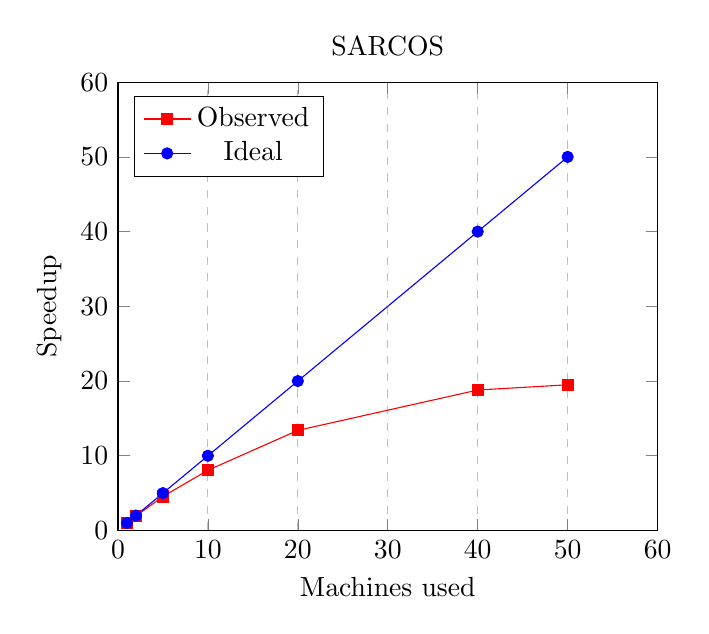
\begin{tikzpicture}
\begin{axis}[title={SARCOS},xlabel={Machines used},ylabel={Speedup},xmin=0, xmax=60,ymin=0, ymax=60,xtick={0,10,20,30,40,50, 60},ytick={0,10,20,30,40,50, 60},legend pos=north west,xmajorgrids=true,grid style=dashed,] 
\addplot[color=red,mark=square*,]
    coordinates {(1,1)(2, 1.94)(5, 4.55)(10, 8.06)(20, 13.4)(40, 18.8)(50, 19.5)};
\addplot[color=blue,mark=*,]
    coordinates {(1,1)(2, 2)(5, 5)(10, 10)(20, 20)(40, 40)(50, 50)};
    \legend{Observed, Ideal}
\end{axis}
\end{tikzpicture}
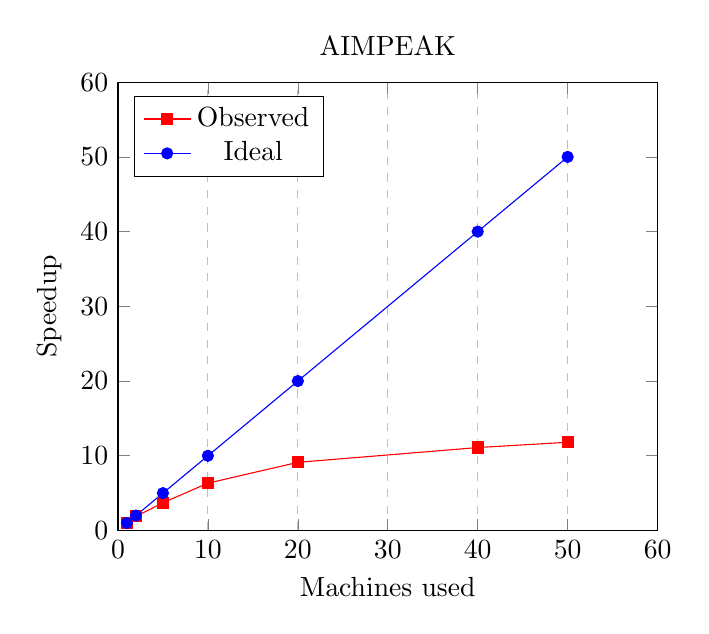
\begin{tikzpicture}
\begin{axis}[title={AIMPEAK},xlabel={Machines used},ylabel={Speedup},xmin=0, xmax=60,ymin=0, ymax=60,xtick={0,10,20,30,40,50, 60},ytick={0,10,20,30,40,50, 60},legend pos=north west,xmajorgrids=true,grid style=dashed,] 
\addplot[color=red,mark=square*,]
    coordinates {(1,1)(2, 1.89)(5, 3.71)(10, 6.33)(20, 9.12)(40, 11.10)(50, 11.81)};
\addplot[color=blue,mark=*,]
    coordinates {(1,1)(2, 2)(5, 5)(10, 10)(20, 20)(40, 40)(50, 50)};
    \legend{Observed, Ideal}
\end{axis}
\end{tikzpicture}
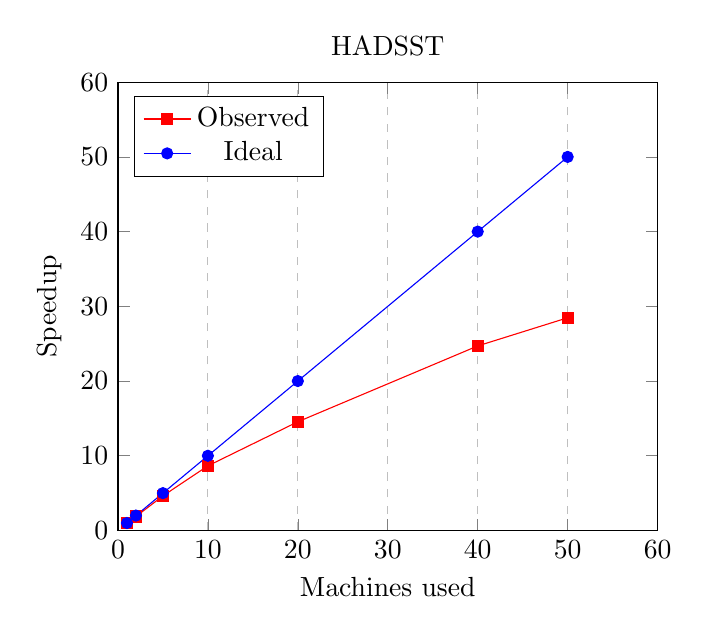
\begin{tikzpicture}
\begin{axis}[title={HADSST},xlabel={Machines used},ylabel={Speedup},xmin=0, xmax=60,ymin=0, ymax=60,xtick={0,10,20,30,40,50, 60},ytick={0,10,20,30,40,50, 60},legend pos=north west,
    xmajorgrids=true,
    grid style=dashed,
] 
\addplot[color=red,mark=square*,]
    coordinates {
    (1,1)(2, 1.87)(5, 4.63)(10, 8.65)(20, 14.55)(40, 24.70)(50, 28.47)};
    \addplot[color=blue,mark=*,]
    coordinates {
    (1,1)(2, 2)(5, 5)(10, 10)(20, 20)(40, 40)(50, 50) };
    \legend{Observed, Ideal}
\end{axis}
\end{tikzpicture}
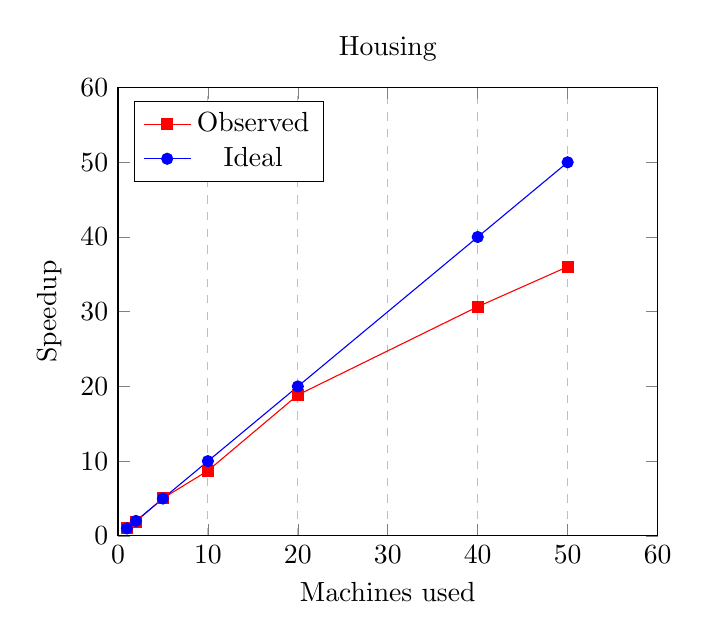
\begin{tikzpicture}
\begin{axis}[title={Housing},xlabel={Machines used},ylabel={Speedup},xmin=0, xmax=60,ymin=0, ymax=60,xtick={0,10,20,30,40,50, 60},ytick={0,10,20,30,40,50, 60},legend pos=north west,
    xmajorgrids=true,
    grid style=dashed,
] 
\addplot[color=red,mark=square*,]
    coordinates {
    (1,1)(2, 1.91)(5, 5.03)(10, 8.72)(20, 18.86)(40, 30.67)(50, 36.02)};
    \addplot[color=blue,mark=*,]
    coordinates {
    (1,1)(2, 2)(5, 5)(10, 10)(20, 20)(40, 40)(50, 50) };
    \legend{Observed, Ideal}
\end{axis}
\end{tikzpicture}
\newline
\centerline{Figure 1. Speedup for various datasets}
\newline\newline
We can make 3 observations from the tabulation and graphs,
\begin{enumerate}[label=(\alph*)]
\item Larger the size of the dataset, larger is the speedup as the number of machines used increases.
\item For all datasets, the speedup begins to decreases after a threshold number of machines are used.
\item For datasets of the same size, the speedup obtained depends on the time for the sequential run (time taken for a single processor to train the dataset).
\end{enumerate}
Points (a) and (b) are analyzed in detail in the following section.\\
The reasoning behind point (c) is intuitive: depending on the nature of the dataset, the number of iterations required for the convergence of the solution varies, and larger number of iterations implies increased training time. Increase in the number of iterations would also mean that the total communication overhead incurred and executions of the sequential portion of the code (see Section \ref{Cholesky Factorization}) increases leading to decrease in speedup.
\newline\newline
{\bf From Figure 1 and Table 2, it can be observed that although the speedup is not ideal, PSVR is able to parallelize the SVR algorithm and scales with increased number of machines used, more effectively so for larger datasets.}
\subsection{Overhead}
\label{Overhead}
From the graphs in Figure 1, we can see that for each of the datasets, the speedups are not ideal, and that the individual speedups vary between datasets.
{\bf The following section attempts to explain the overheads incurred by PSVR which affect the overall speedup of the process.}
\newline\newline
Usage of parallel computing in PSVR incurs two types of overheads, Communication overhead and Synchronization overhead.
\begin{itemize}
\item Communication overhead corresponds to the overhead incurred due to broadcast and transmission of messages over the network as part of MPI. 
\newline
As the number of machines used increases, the communication over the network at each step increases as well, implying more Communication overhead with increase number of machines.The increase in overhead could be minimal\footnotemark or substantial depending on the underlying architecture of the supercomputing cluster.
 \footnotetext{In Figure 2, we notice that the Communication overhead rises significantly until m = 5 and then the increase is minor; The collective operations using MPI3 are substantially faster for processors on the same physical machine (since network traffic is minimized) and after m $\geq$ 5, while the number of processors per physical machines used increases, the number of physical machines used remains the same, causing the overhead to increase minimally for subsequent values of m(since inter-processor communication does not rely on the network).}
\item Synchronization overhead occurs due to non-identical configuration of the machines used. Various machines are capable of executing the program at various speeds and after each step in PSVR, a synchronization occurs (using MPIBarrier) which ensures that every machine has reached the same point of execution (to prevent the situation that one of the machines fails but the other machines aren't notified).
\end{itemize}
The graphs below plot the Communication and Synchrnoization overhead for each of the datasets using varying number of machines.

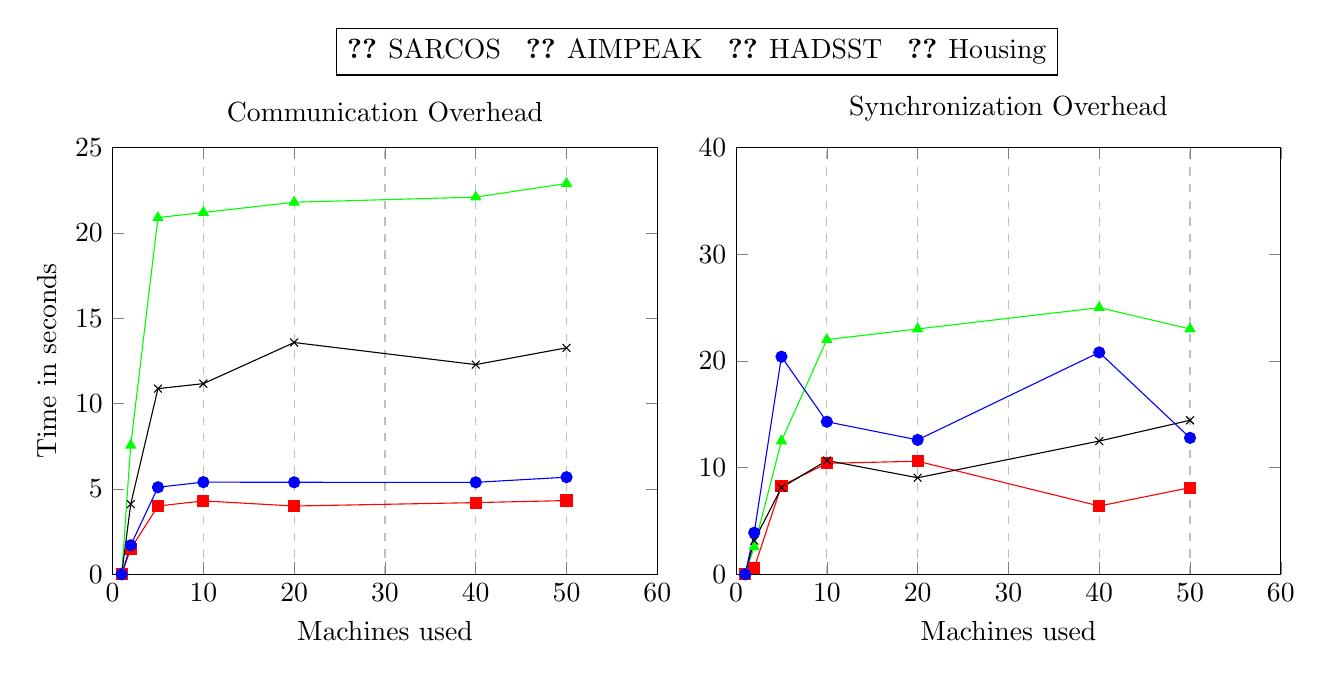
\begin{tikzpicture}
 \begin{groupplot}[group style={group size= 2 by 1},height=7cm,width=8.5cm]
  \nextgroupplot [title={Communication Overhead},xlabel={Machines used},xmin=0, xmax=60,ymin=0, ymax=25,xtick={0,10,20,30,40,50, 60},ytick={0,5,10,15,20, 25},legend style={at={(0.5,0.5)},anchor=west},xmajorgrids=true,grid style=dashed,] 
\addplot[color=red,mark=square*,]
    coordinates {
    (1,0)(2, 1.49)(5, 4)(10, 4.3)(20, 4)(40, 4.2)(50, 4.32)
    };
    \label{plots:sarcos}
    \addplot[color=green,mark=triangle*,]
    coordinates {(1,0)(2, 7.56)(5, 20.9)(10, 21.2)(20, 21.8)(40, 22.1)(50, 22.9)};
    \label{plots:aimpeak}
     \addplot[color=black,mark=x,]
    coordinates {(1,0)(2, 4.11)(5, 10.88)(10, 11.17)(20, 13.58)(40, 12.286)(50, 13.27)};
    \label{plots:hadsst}
    \addplot[color=blue,mark=*,]
    coordinates {
    (1,0)(2, 1.7)(5, 5.1)(10, 5.4)(20, 5.39)(40, 5.388)(50, 5.69)
    };
    \label{plots:housing}
    \coordinate (top) at (rel axis cs:0,1);% coordinate at top of the first plot
    \nextgroupplot [title={Synchronization Overhead},xlabel={Machines used},,xmin=0, xmax=60,ymin=0, ymax=40,xtick={0,10,20,30,40,50, 60},ytick={0, 10,20, 30, 40},legend pos=north west,xmajorgrids=true,grid style=dashed,] 
\addplot[color=red,mark=square*,]coordinates {(1,0)(2, 0.62)(5, 8.3)(10, 10.4)(20, 10.6)(40, 6.4)(50, 8.12)};
\addplot[color=green,mark=triangle*,]
coordinates {(1,0)(2, 2.57)(5, 12.5)(10, 22)(20, 23)(40, 25)(50, 23)};
 \addplot[color=black,mark=x,]
    coordinates {(1,0)(2, 3.16)(5, 8.12)(10, 10.67)(20, 9.05)(40, 12.49)(50, 14.44)};
\addplot[color=blue,mark=*,]
 	coordinates {(1,0)(2, 3.9)(5, 20.4)(10, 14.3)(20, 12.6)(40, 20.8)(50, 12.79)};
 	\coordinate (bot) at (rel axis cs:1,0);% coordinate at bottom of the last plot
\end{groupplot}
 \path (top-|current bounding box.west)-- 
          node[anchor=south,rotate=90] {Time in seconds} 
          (bot-|current bounding box.west);
% legend
\path (top|-current bounding box.north)--
      coordinate(legendpos)
      (bot|-current bounding box.north);
\matrix[
    matrix of nodes,
    anchor=south,
    draw,
    inner sep=0.2em,
    draw
  ]at([yshift=1ex]legendpos)
  {
    \ref{plots:sarcos}& SARCOS&[5pt]
    \ref{plots:aimpeak}& AIMPEAK &[5pt]
    \ref{plots:hadsst}& HADSST & [5pt]
    \ref{plots:housing}& Housing\\};
\end{tikzpicture}
\newline
\centerline{Figure 2. Overheads incurred for datasets}
\newline\newline
We can make certain observations from these graphs.
\begin{enumerate}[label=(\alph*)]
\item For the larger dataset, although both the overheads are comparable to that of the smaller datasets, the speedup is affected less due to the fact that the computational time for the program is much more than the time for the overheads.
\item We also observe that for the SARCOS and AIMPEAK datasets (which have approximately the same number of training instances,), there is significant difference in the overhead, and therefore the speedups. This is due to the nature if the datasets; The SARCOS dataset converges to a solution in much fewer iterations than the AIMPEAK dataset, causing the AIMPEAK dataset to incur much more overhead due to increased number of iterations.
\end{enumerate}
\subsubsection{Sequential Cost}	
A cost not considered until now is the cost for the sequential part of the program i.e Cholesky Factorization(Section \ref{Cholesky Factorization}). As mentioned above, the cost for Cholesky Factorization is incurred for every IPM iteration and is dependent only on the square of the reduced rank of the matrix, $p^2$. Since the process is non-parallelizable, the overhead will be constant for the PSVR process for a particular dataset, independent of the number of machines used.
\newline The graphs below plot the observed speedup, speedup without the Cholesky Factorization(CF) and the ideal speedup.
\newline
\newline
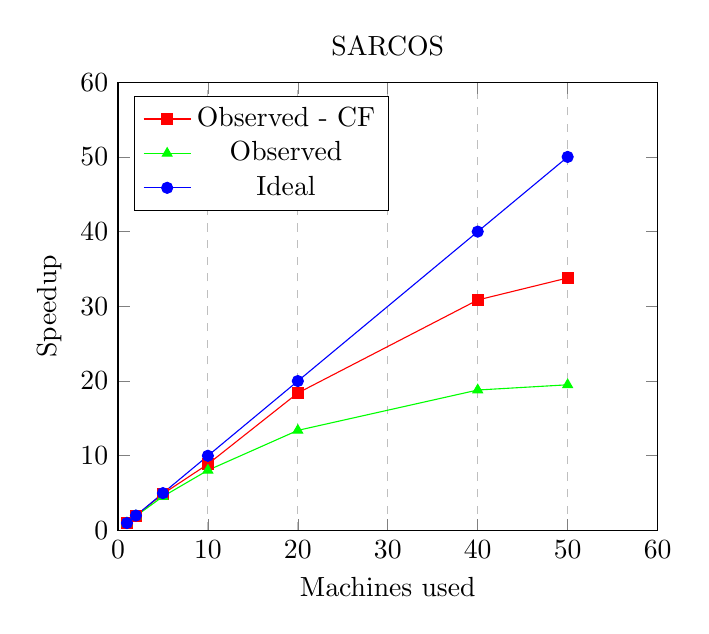
\begin{tikzpicture}
\begin{axis}[title={SARCOS},xlabel={Machines used},ylabel={Speedup},xmin=0, xmax=60,ymin=0, ymax=60,xtick={0,10,20,30,40,50, 60},ytick={0,10,20,30,40,50, 60},legend pos=north west,xmajorgrids=true,grid style=dashed,] 
\addplot[color=red,mark=square*,]
    coordinates {
    (1,1)(2, 1.99)(5, 4.90)(10, 8.88)(20, 18.40)(40, 30.85)(50, 33.80)
    };
    \addplot[color=green,mark=triangle*,]
    coordinates {(1,1)(2, 1.94)(5, 4.55)(10, 8.06)(20, 13.4)(40, 18.8)(50, 19.5)};
    \addplot[color=blue,mark=*,]
    coordinates {
    (1,1)(2, 2)(5, 5)(10, 10)(20, 20)(40, 40)(50, 50)
    };
    \legend{Observed - CF, Observed, Ideal}
\end{axis}
\end{tikzpicture}
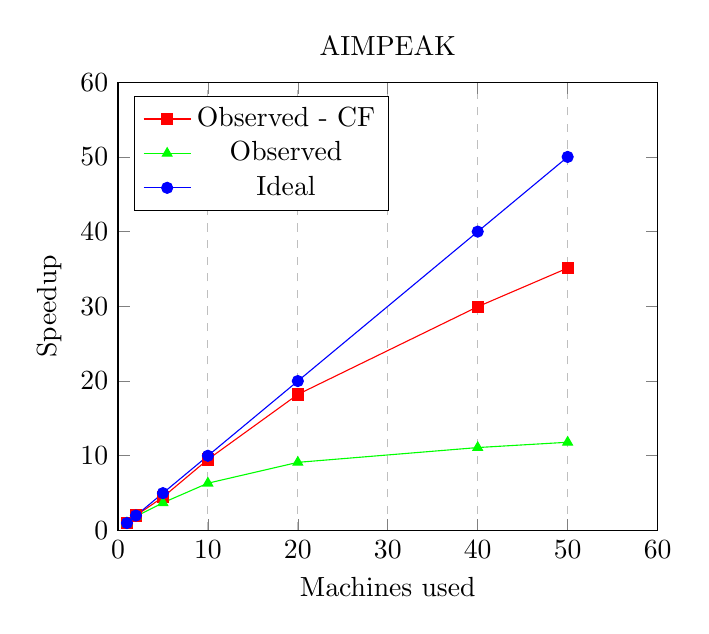
\begin{tikzpicture}
\begin{axis}[title={AIMPEAK},xlabel={Machines used},ylabel={Speedup},xmin=0, xmax=60,ymin=0, ymax=60,xtick={0,10,20,30,40,50, 60},ytick={0,10,20,30,40,50, 60},legend pos=north west,xmajorgrids=true,grid style=dashed,] 
\addplot[color=red,mark=square*,]coordinates {(1,1)(2, 2)(5, 4.46)(10, 9.51)(20, 18.21)(40, 29.95)(50, 35.12)};
\addplot[color=green,mark=triangle*,]
coordinates {(1,1)(2, 1.89)(5, 3.71)(10, 6.33)(20, 9.12)(40, 11.10)(50, 11.81)};
\addplot[color=blue,mark=*,]
 	coordinates {(1,1)(2, 2)(5, 5)(10, 10)(20, 20)(40, 40)(50, 50)};
    \legend{Observed - CF, Observed, Ideal}
\end{axis}
\end{tikzpicture}
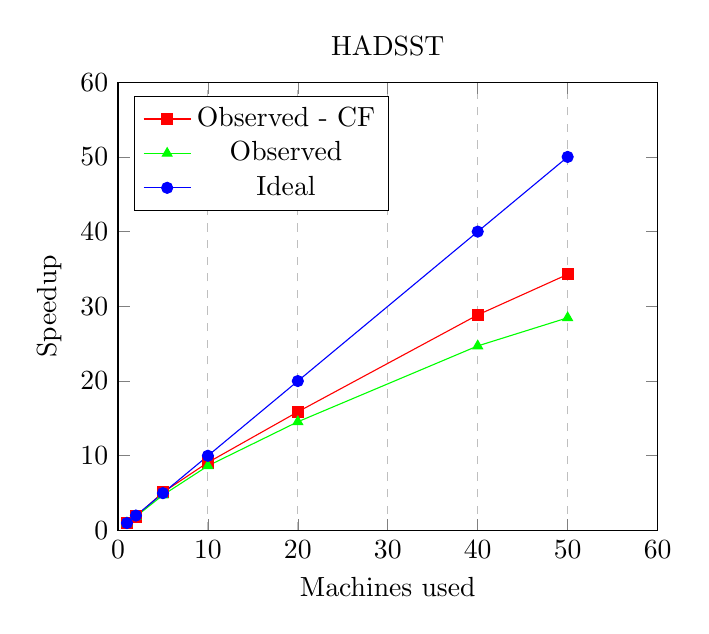
\begin{tikzpicture}
\begin{axis} [title={HADSST},xlabel={Machines used},ylabel={Speedup},xmin=0, xmax=60,ymin=0, ymax=60,xtick={0,10,20,30,40,50, 60},ytick={0,10,20,30,40,50, 60},legend pos=north west,xmajorgrids=true,grid style=dashed,] 
\addplot[color=red,mark=square*,]coordinates {(1,1)(2, 1.88)(5, 5.10)(10, 9.1)(20, 15.88)(40, 28.85)(50, 34.28)};
\addplot[color=green,mark=triangle*,] coordinates {(1,1)(2, 1.87)(5, 4.74)(10, 8.65)(20, 14.55)(40, 24.70)(50, 28.47)};
\addplot[color=blue,mark=*,]
 	coordinates {(1,1)(2, 2)(5, 5)(10, 10)(20, 20)(40, 40)(50, 50)};
    \legend{Observed - CF, Observed, Ideal}
\end{axis}
\end{tikzpicture}
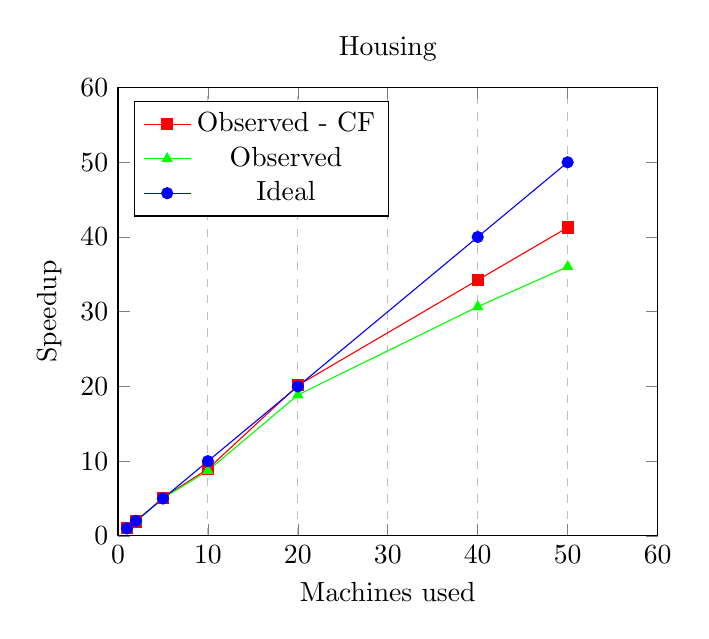
\begin{tikzpicture}
\begin{axis} [title={Housing},xlabel={Machines used},ylabel={Speedup},xmin=0, xmax=60,ymin=0, ymax=60,xtick={0,10,20,30,40,50, 60},ytick={0,10,20,30,40,50, 60},legend pos=north west,xmajorgrids=true,grid style=dashed,] 
\addplot[color=red,mark=square*,]coordinates {(1,1)(2, 1.92)(5, 5.10)(10, 8.96)(20, 20.14)(40, 34.24)(50, 41.27)};
\addplot[color=green,mark=triangle*,] coordinates {(1,1)(2, 1.91)(5, 5.03)(10, 8.72)(20, 18.86)(40, 30.67)(50, 36.02)};
\addplot[color=blue,mark=*,]
 	coordinates {(1,1)(2, 2)(5, 5)(10, 10)(20, 20)(40, 40)(50, 50)};
    \legend{Observed - CF, Observed, Ideal}
\end{axis}
\end{tikzpicture}
\ \\
\centerline{Figure 3. Speedup for various datasets excluding Synchronous component.}
\newline\newline
From these graphs, we still see that none of these speedup curves follow the ideal speedup curve. The deviation from the ideal speedup in these graphs is due to the Synchronization and Communication overheads.
\newline\newline
From these graphs, we can also make certain observations regarding the nature of the speedup curve.
\begin{enumerate}[label=(\alph*)]
\item With fewer machines, this effect of the Cholesky Factorization portion is not observed as the time taken for this computation is insignificant when compared to the time taken for the overall computation. As the number of machines used increases, the time taken for computation of other portions decreases (nearly linearly) while the time for executing the Cholesky Factorization remains the same, making the cost of the sequential portion significant.
\item For smaller datasets, the speedup deteriorated at a much faster rate as compared to the larger ones, when the Cholesky Factorization was included. For smaller datasets, the time for each iteration (and overall time) is much smaller than for the larger datasets and so, by using a few machines $(m < 40)$, the time taken for all portions of the program except the sequential portions reduces quickly. This means that even with a few machines, the time taken for the sequential portion of the program becomes significant and reduces the speedup achieved. For larger datasets, this same effect of the sequential portion of the program is not observed until several more machines are used as the time taken for the execution of the sequential portion is insignificant compared to the time taken for the execution for the rest of the algorithm in each iteration when only a few machines are used.
\end{enumerate}
From Amdahl's law, the speedup that can be achieved is capped by the un-parallelizable portions of the program. From our results and observations above, this means that for a larger speedup, the time taken for the un-parallelizable portion of the program needs to be insignificant compared to the rest of the program, which is the case for larger datasets. So, {\bf larger the dataset, greater is the speedup we can achieve by increasing the machines used.} For smaller datasets, since the time taken for the un-parallelizable portion of the program is not insignificant, the speedup that can be achieved will be limited.
\subsection{Summary of Results}
\label{Summary of Results}
From the observations in the previous subsections, we can make certain observations:
\begin{enumerate}[label=(\alph*)]
\item {\bf PSVR successfully parallelizes SVR algorithm}
\newline
The following observation can be made from Table 2; For a given dataset, PSVR can effectively parallelize the SVR algorithm to provide increased speedup with increasing number of machines used. The speedup achieved with increasing number of machines is nearly linear, except for the overheads detailed in Section \ref{Overhead}. This would  mean that the PSVR algorithm can be scaled almost linearly (by using more machines) to be used with larger datasets which correspond to real-world data.

\item {\bf Predictive performance of PSVR nearly equivalent to existing state-of-the-art}
\newline
In Table 1, we compare the predictive performance of PSVR to that of the state-of-the-art SVR implementation(LIBSVM) and observe that for each of the datasets, the predictive performance of PSVR is nearly equivalent to that of LIBSVM even with the Kernel Matrix approximation.
\newline
The rank-ratio($p/n$) of the approximated Kernel Matrix, utilized to achieve a nearly equivalent predictive performance, is dependent on the size of the dataset. As the size of the dataset increases, the rank-ratio of the approximated matrix used decreases. This means for larger datasets, the size of the matrix to actually be considered will be smaller.

\item {\bf PSVR outperforms existing state-of-the-art with respect to computational time}
\newline
In Table 2, we also tabulate the time taken for the state-of-the-art (LIBSVM) and notice that the time taken for PSVR to compute the solution, in most cases, is much less than that for LIBSVM. For larger datasets, the computational time is significantly less for each setting of machines used. 
\newline
For smaller datasets, this is not always the case; LIBSVM outperforms PSVR when run on only one machine, but with parallelization PSVR converges to a solution much faster than LIBSVM. The reason for LIBSVM initially outperforming PSVR is that LIBSVM is better equipped to handle smaller datasets and can perform several optimizations (Kernel Caching) to speed up performance. These optimizations do not scale well with larger datasets. When parallel machines are used, the PSVR process speeds up nearly linearly to decrease the time taken for computation.
\end{enumerate}
\cleardoublepage
\section{Conclusion}
Through the course of this paper, we have highlighted the salient features of Support Vector Regression and identified the need for a SVR implementation that allows usage of large datasets. Following this, a novel Parallel Support Vector Regression(PSVR) algorithm was proposed which  allowed the SVR convex optimization problem to be efficiently solved by reducing the initial memory requirement from $O(n^2)$ to $O(np/m)$ and the computational complexity from $O(n^3)$ to $O(np^2/m)$,  where $m$ is the number of machines available, $n$ is the number of training instance and $p$ is the reduced matrix dimension with $p << n$. PSVR  achieves this through a combination of distributing the computational load among parallel machines and performing a matrix approximation of the Kernel matrix.
\newline\newline
The proposed PSVR algorithm was then implemented in C++ using the Message Parsing Interface and through experiments we verified that PSVR outperformed the state-of-the-art SVR implementation with respect to computational complexity in almost all cases. We also verified that PSVR had nearly equivalent predictive accuracy as the state-of-the-art implementations. The overheads associated with the PSVR algorithm and implementation were also explained and supported by the results of the experiments. 
\newline
\newline
{\bf Through the course of these experiments, we could firmly establish that Parallel Support Vector Regression effectively solves the scalability issues associated with Support Vector Regression for usage with larger datasets.}
\newline
\newline
This being said, although PSVR is effective and can be used for smaller datasets, LIBSVM and other SVR implementations which have been specifically optimized for smaller datasets maybe a better option, if a insufficient number of parallel machines are available. For larger datasets, PSVR outperforms LIBSVM even if only a single machine is used and is the clear choice for usage.
\newline\newline
The PSVR implementation is available at \url{https://github.com/akshayv/psvr}. 
\subsection{Future Improvements}
The PSVR project still has potential for improvements, the most salient of which being:
\begin{itemize}
\item A pre-processing step could be introduced to determine the optimal parameter values for the SVR training process, possibly through maximum likelihood estimates. The importance of this feature stems from the fact that the tuning of parameters in the SVR process makes a significant difference in the predictive accuracy and re-training the entire model to find the optimal parameter values would significantly increase the computational time.
\item One of the requirements for both the Incomplete Cholesky Factorization and Cholesky Factorization processes is that the matrix to be factorized be a symmetric, positive-definite matrix and the matrices generated by using the standard Kernel Functions satisfy this criteria. There exists an extension of the standard Radial Basis Kernel Function which allows varying the hyperparameters for each of the input features to provide a more accurate regression model. Unfortunately, the Kernel matrix that is constructed from this modified function does not satisfy the conditions of a positive semi-definite matrix. Using a smaller rank ratio to approximate this matrix provides worse results compared to matrix generated by the standard Kernel Functions with the same rank ratio. This issue can be alleviated by using a large rank ratio for the approximated matrix, but this would incur a larger computational cost in the process of performing a Cholesky factorization, so is currently sub-optimal. Resolving this issue would improve predictive performance of PSVR (although not significantly).
\end{itemize}
\cleardoublepage
\pagenumbering{roman}
\setcounter{page}{\value{reportpage}}
\section{Appendix}
\subsection{A: Parallel Incomplete Cholesky factorization }
ICF can approximate $Q (Q \in R^{n\times n})$ by a smaller matrix $H (H \in R^{n\times p},p \ll n)$, i.e., $Q \approx HH^T$.
Our row-based parallel ICF (PICF) works as follows: Let vector $v$ be the diagonal of $Q$ and suppose the pivots (the largest diagonal values) are $\{i_1, i_2, . . . , i_k\}$, the $k^{th}$ iteration of ICF computes three
equations:
\begin{gather}
H(i_k, k) = \sqrt{v(i_k)}\\
H(J_k, k) = \frac{(Q(J_k, k) - \sum_{j=1}^{k-1}{H(J_k, j)(H(i_k, j))}}{H(i_k, k)}\\
v(J_k) = v(J_k) - H(J_k, k)^2, 
\end{gather}
where $J_k$ denotes the complement of $\{i_1 , i_2 , . . . , i_k \}$. The algorithm iterates until the approximation of $Q$ by $H_k H_ k^T$ (measured by $trace(Q − H_k H_k^T )$) is satisfactory, or the predefined maximum iterations (or say, the desired rank of the ICF matrix) p is reached.\newline
\newline
{\bf The details of computing the pivots and updating the vectors in each iteration have been explained in Algorithm 1.}
\newline
At the end of the algorithm, $H$ is stored distributedly on $m$ machines, ready for parallel IPM. PICF enjoys three advantages: parallel memory use $(O(np/m))$, parallel computation $(O(p^2n/m))$, and low communication overhead $(O(p^2 log(m)))$. 

\begin{algorithm}
\caption{Row-based PICF}
\begin{algorithmic} [1]

\STATEx {\bf Input} $n$ training instances; $p$: rank of ICF matrix H; $m$: number of machines
\STATEx {\bf Output} $H$ distributed on $m$ machines
\STATEx{\bf Variables:}
\STATEx $v$: fraction of the diagonal vector of $Q$ that resides in local machine
\STATEx $k$: iteration number;
\STATEx $x_{i}$: the $i$th training instance
\STATEx $M$: machine index set, $M = {0,1,...,m - 1}$
\STATEx $I_{c}$: row-index set on machine $c$ $(c \in M)$, $I_{c} = {c,c + m,c + 2m,...}$

\FOR {$i=0$ to $n-1$}
\STATE Load $x_{i}$ into machine $imodulom$.
\ENDFOR
\STATE $k \leftarrow 0; H \leftarrow 0; v \leftarrow$  the fraction of the diagonal vector of $Q$ that resides in local machine.$ (v(i)(i \in I_{m})$ can be obtained from $x_{i}$).
\STATE Initialize $master$ to be machine $0$.
\WHILE{$k < p$}
\STATE Each machine $c \in M$ selects its local pivot value, which is the largest element in $v$:
\STATEx \centerline{$\bm{lpv_{k,c}} =max\ \bm{v(i)}, i\in I_{c}$.}
\STATEx and records the local pivot index, the row index corresponds to $\bm{lpv_{k,c}}$:
\Statex  \centerline{$\bm{lpi_{k,c}} =arg\ max\ \bm{v(i)}, i\in I_{c}$.}
\STATE Gather $\bm{lpv_{k,c}}$’s and $\bm{lpi_{k,c}}$’s $(c \in M)$ to $master$.
\STATE The $master$ selects the largest local pivot value as global pivot value $\bm{gpv_{k}}$ and records in $i_{k}$, row index corresponding to the global pivot value.
\Statex  \centerline{$\bm{gpv_{k}} =max\ \bm{lpv_{k,c}},  c \in M$}
\STATE The master broadcasts $\bm{gpv_{k}}$ and $i_{k}$.
\STATE Change $master$ to machine $i_{k}\%m$.
\STATE Calculate $H(i_{k}, k)$ according to (10) on master.
\STATE The $master$ broadcasts the pivot instance $x_{i_{k}}$ and the pivot row $H(i_{k},:)$. (Only the first $k+1$ values of the pivot row need to be broadcast, since the remainder are zeros.)
\STATE Each machine $c \in M$ calculates its part of the $k$th column of $H$ according to (11).
\STATE Each machine $c \in M$ updates $v$ according to (12).
\STATE $k \leftarrow k+1$
\ENDWHILE
\end{algorithmic}
\end{algorithm}


\cleardoublepage

\section{References}
\renewcommand{\section}[2]{}%
 \begin{thebibliography}{}
 
  \bibitem{svrtut}Smola A.,  Scholkopf B. {\em A Tutorial on Support Vector Regression} 2004:  Statistics and computing 14.3: 199-222.
  
 \bibitem{esl}Hastie T. {\em Elements of Statistical Learning} 2009:  Vol. 2. No. 1. New York: Springer.
    
 \bibitem{svrthesis}Smola A. {\em Regression
Estimation with Support Vector Learning Machines} 1996: Master's thesis, Technische Universit at Munchen.


\bibitem{nu-svm}Sch\"olkopf, B., A. J. Smola, and R. Williamson. {\em Shrinking the tube: A new support vector regression algorithm} 1999: In M. S. Kearns, S. A. Solla, and 22 D. A. Cohn (Eds.), Advances in Neural Information Processing Systems, Volume 11, Cambridge, MA. MIT Press

\bibitem{}Bekkerman, R., Bilenko, M., and Langford, J. {\em Scaling up Machine Learning: Parallel and Distributed Approaches} 2011: Cambridge Univ. Press, NY.

 \bibitem{psvm}Chang E., Zhu K., Wang H., Bai H.  {\em PSVM: Parallelizing Support Vector Machines on Distributed Computers} 2007: In Proc. NIPS.
 
 \bibitem{psvm1} Wu G., Chang E., Chen Y.K., Hughes C.  {\em Incremental Approximate Matrix Factorization for Speeding up Support Vector Machines} 2006: Proceedings of the 12th ACM SIGKDD international conference on Knowledge discovery and data mining. ACM.

 \bibitem{pgp} Chen J., Cao N., Low K. H.,  Ouyang R., Tan C. K., Jaillet P.  {\em Parallel Gaussian Process Regression with Low-Rank Covariance Matrix Approximations} 2013: arXiv preprint arXiv:1305.5826
 
\bibitem{SMO}J. C. Platt {\em Fast training of support vector machines using sequential minimal optimization} 1999: Advances in kernel methods: support vector learning, pp. 185–208

\bibitem{kernelcaching}T. Joachims. {\em Making large-scale support vector machine learning practical} 1999: Advances in kernel methods: support vector learning, pp. 169–184

\bibitem{chunkingsvr}E. Osuna, R. Freund, and F. Girosi. {\em Training support vector machines: an application to face detection} 1997: In Proceedings of the 1997 Conference on Computer Vision and Pattern Recognition, pp. 130–136

\bibitem{mrpsvm}H. X. Zhao, F. Magoules. {\em New parallel support vector regression for predicting building energy consumption}.2011: IEEE Symposium Series on Computational Intelligence (SSCI 2011), Paris, France. IEEE Computer Society

 \bibitem{cassvm} Graf, H. P., Cosatto, E., Bottou, L., Dourdanovic, I., Vapnik, V.  {\em Parallel Support Vector Machines: The Cascade SVM} 2005: In Advances in neural information processing systems 17, 521-528

\bibitem{picf} Golub, G. H., Loan, C. F. V. {\em Matrix computations} 1996: Johns Hopkins University Press.

  \bibitem{convoptme} Mehrotra S.  {\em On the implementation of a primal-dual interior point method} 1992: SIAM J. Optimization, 2.

 \bibitem{convopt}Boyd S. {\em Convex optimization}  2004: Cambridge University Press.
  
  \bibitem{ipmsvm}Woodsend K. {\em Using Interior Point Methods for Large-scale Support Vector Machine training} 2010
  
\bibitem{libsvm-soa}Lin C., Bottou L. {\em Support Vector Machine Solvers} 2005: MIT Press

\bibitem{SARCOS}Vijayakumar, S., D’Souza, A., and Schaal, S. {\em Incremental online learning in high dimensions} 2005: Neural Comput., 17(12), pp 2602–2634.


  \end{thebibliography}
 \end{document}